% Use class option [extendedabs] to prepare the 1-page extended abstract.
\documentclass[extendedabs]{bmvc2k}
\usepackage[colorlinks = true,
            linkcolor = blue,
            urlcolor  = blue,
            citecolor = blue,
            anchorcolor = blue]{hyperref}
\graphicspath{ {figures/} }

% Document starts here
\begin{document}


\title{Enriching Object Detection with 2D-3D Registration and Continuous Viewpoint Estimation}
\addauthor{
Christopher Bongsoo Choy\textsuperscript{\dag}, Michael Stark\textsuperscript{\dag \ddag}, Sam Corbett-Davies\textsuperscript{\dag}, Silvio Savarese\textsuperscript{\dag}}{}{1}
\addinstitution{
\textsuperscript{\dag}Stanford University, \textsuperscript{\ddag}Max Planck Institute for Informatics
}


\maketitle
\let\thefootnote\relax\footnote{This is an extended abstract. The full paper is available at the \href{http://www.cv-foundation.org/openaccess/CVPR2015.py}{Computer Vision Foundation webpage}. }
\vspace{-0.2in}


% Extended abstract begins here.  In a one-page document, there is
% little need for section headers, but you may use \section etc if you
% wish.

\begin{figure}[t]
  \centering
  % 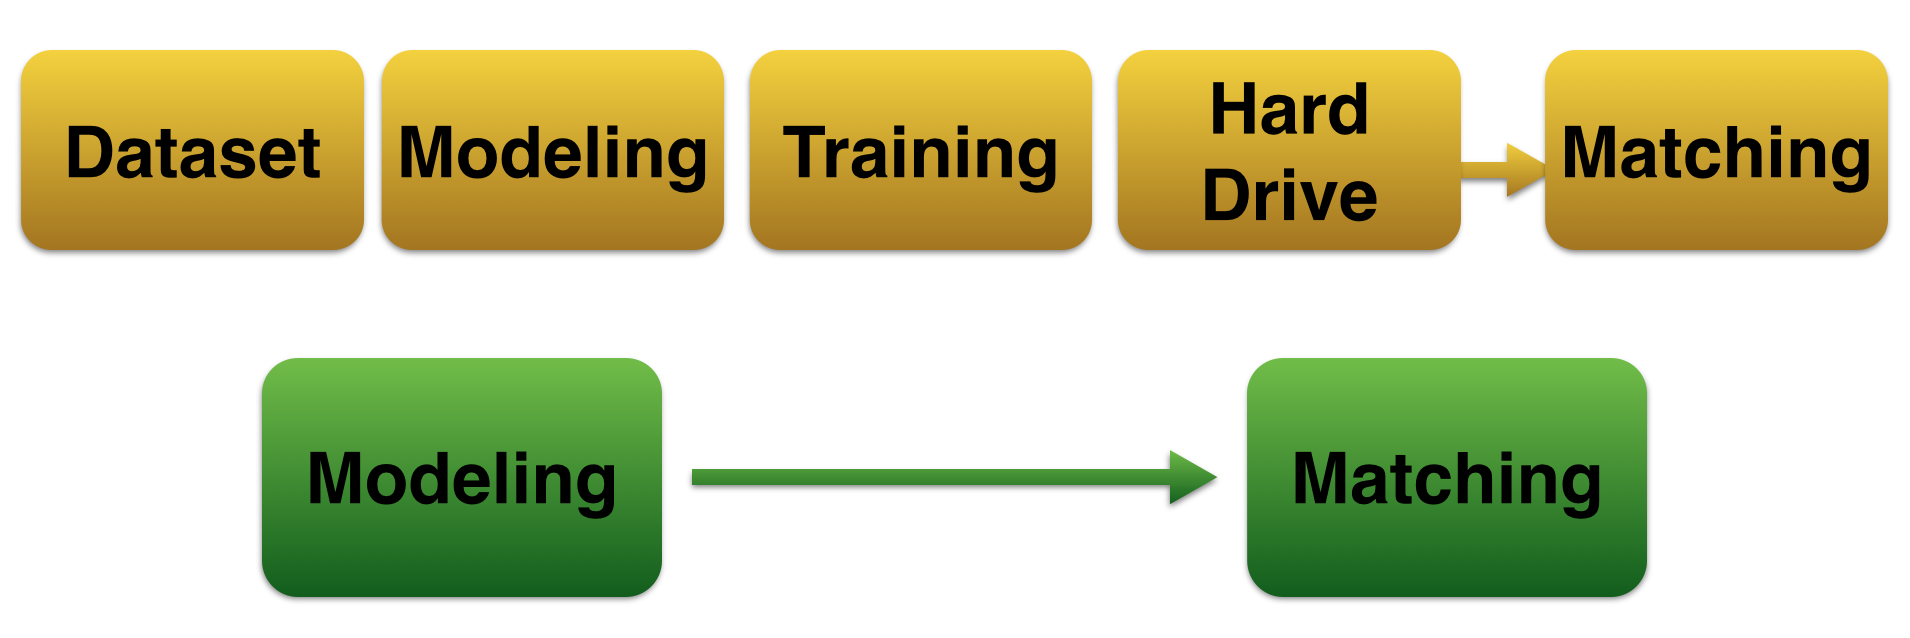
\includegraphics[width=0.9\linewidth]{schematics} 
  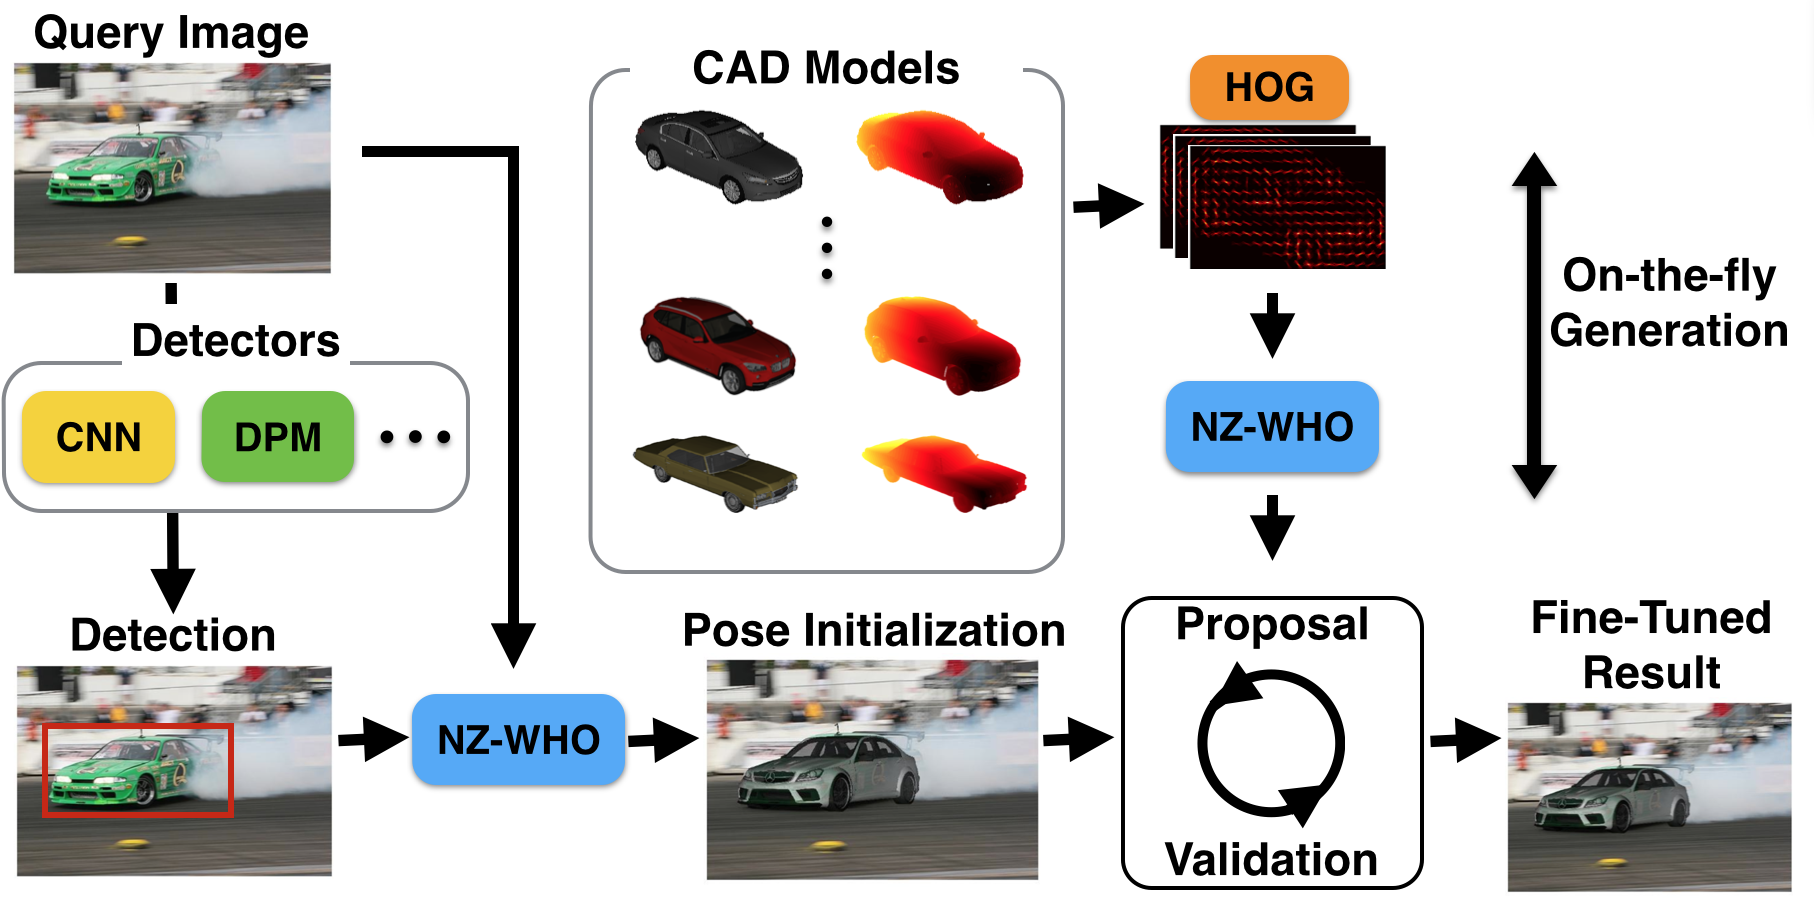
\includegraphics[width=0.9\linewidth]{front} % \\[-5pt]
  \caption{Using a database of 3D CAD models, we generate NZ-WHO
    templates which can be used to either detect objects directly or
    enrich the output of an existing detector with high-quality,
    continuous pose and 3D CAD model exemplar.}
    % initialize pose of an object in the bounding box from other
    % detectors. Once initialization is given, we use NZ-WHO to propose
    % and validate plausible pose on-the-fly and
    % further tune the translation, 3D viewpoint and focal length continuously.}
  % \vspace{-1em}
  \label{fig:front}
\end{figure}
\vspace{-0.15in}

% In this paper, we propose a novel method for 2D-3D alignment of exemplar CAD
% models to real-world images that circumvents the need for calibration and
% greatly enhances the scalability of WHO. Our model generates a discriminative
% exemplar template on-the-fly and align model accurately using MCMC.

\noindent
A large body of recent work on object detection has focused on providing more
information than the bounding box of an object. One set of methods use 3D CAD
model databases to provide viewpoint estimation. These approaches work
by aligning exact 3D models to images using templates generated from renderings
of the 3D models at a set of discrete viewpoints~\cite{Aubry14}.

However, training templates for all viewpoints and CAD models is not feasible
since it requires a huge amount of training data to be acquired. Instead, it has been realized that template-based exemplar
detectors based on HOG features can be trained analytically, by
replacing the standard SVM with an LDA classifier $w_{x_t}$ for a template $x_t$
~\cite{Hariharan12}.

The result is a whitened feature representation, termed WHO (Whitened Histogram
of Orientations). This development makes it feasible to train a large number of
mid-level patch detectors for recognition.

Though generating and calibrating LDA templates (via matrix decomposition with
Gaussian Elimination) achieved remarkable improvements, they are
computationally expensive and use a prohibitive amount of memory and storage.
In addition, viewpoint discretization hampers pose estimation performance.

% In this paper, instead of caching and calibrating all templates on training
% time, we selectively generate templates on testing time as well to estimate
% viewpoint continuously using the technique we proposed termed Non-Zero Whitened
% Histograms of Orientations (NZ-WHO).

% The method uses Conjugate Gradient method to efficiently generate an LDA template on-the-fly (60 ms) without expensive calibration steps.

\vspace{-0.15in}
\paragraph{Overview.} In this paper, we propose a novel method for 2D-3D
alignment of exemplar CAD models to real-world images that circumvents the need
for calibration and greatly enhances the scalability of WHO. As a result, we
can render novel views and train corresponding exemplar models {\em
	on-the-fly}, without the need for offline processing. We call these Non-Zero
Whitened Histograms of Orientations (NZ-WHO) templates. To our knowledge, our
method constitutes the first attempt to simultaneously render and train
exemplar detectors on-the-fly.

First, we adapt the whitening to the specific case of rendered images. We show
how to speed up the whitening by two orders of magnitude for high-resolution
templates using Conjugate Gradient method. Also, we improve the evaluation of
our 3D exemplar template detectors at test time by performing convolutions in
the frequency domain.

These components make template generation and evaluation computationally
inexpensive. Thus, we are able to efficiently explore the continuous parameter
space to find the best object pose, scale, 3D CAD model type and camera focal
length. An overview of our pipeline can be seen in Fig.~\ref{fig:front}.

Finally, our experimental study demonstrates the effectiveness of the
approach on several standard benchmarks for object detection and viewpoint
estimation. We also demonstrate that our method can enrich the output of an
existing object class detector, such as DPM or R-CNN, with additional 3D
information.

\begin{figure}[t]
\small
\setlength\tabcolsep{1pt}
\centering
\begin{tabular}{ccccc}
  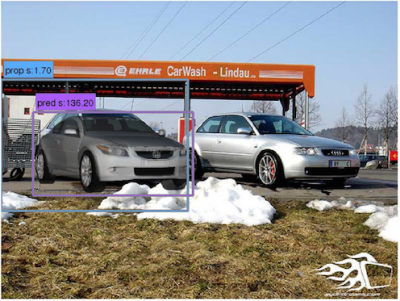
\includegraphics[width=0.18\textwidth]{car_cnn/2c.png} &
  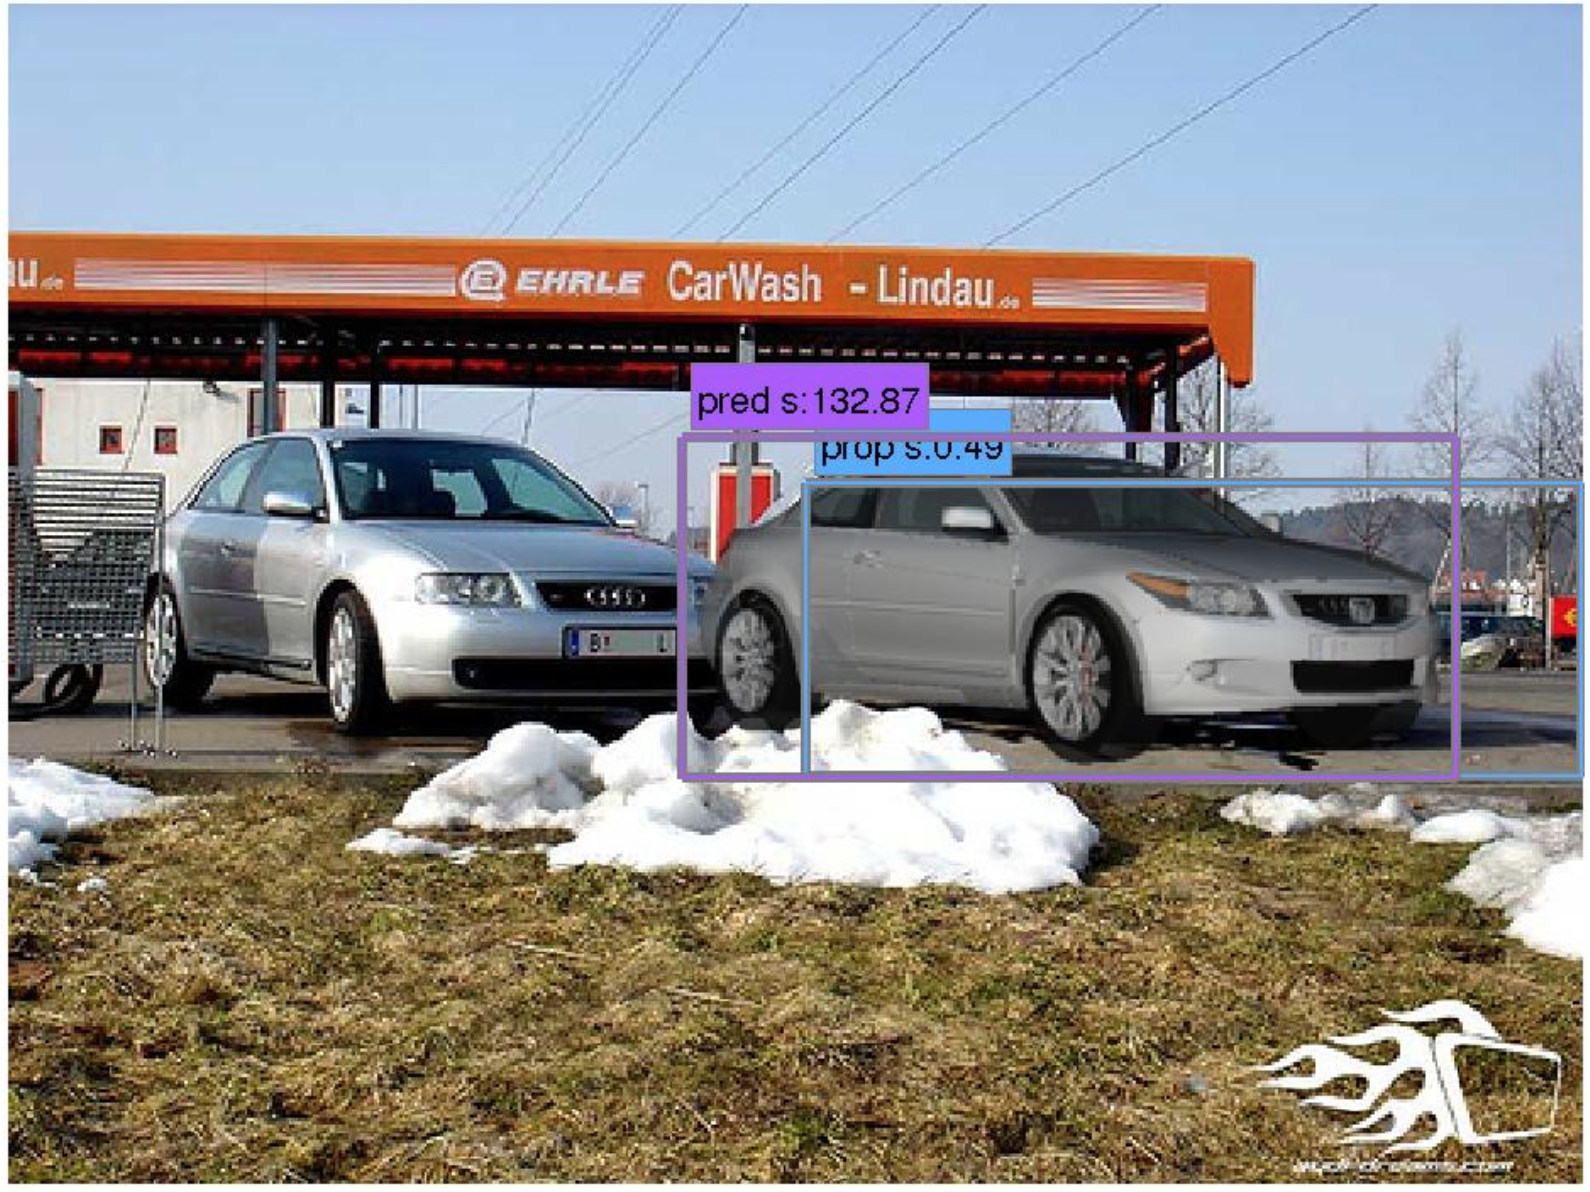
\includegraphics[width=0.18\textwidth]{car_cnn/2e.png} \\
  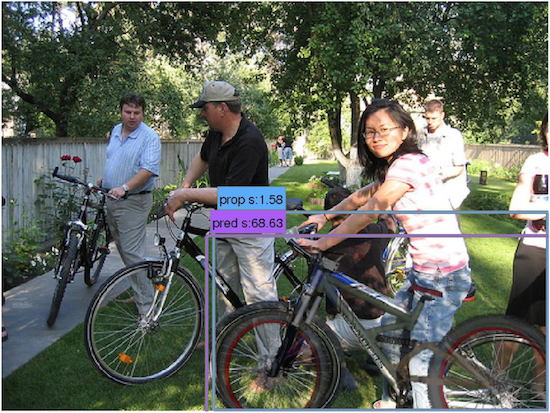
\includegraphics[width=0.18\textwidth]{bicycle_cnn/4b.png} &
  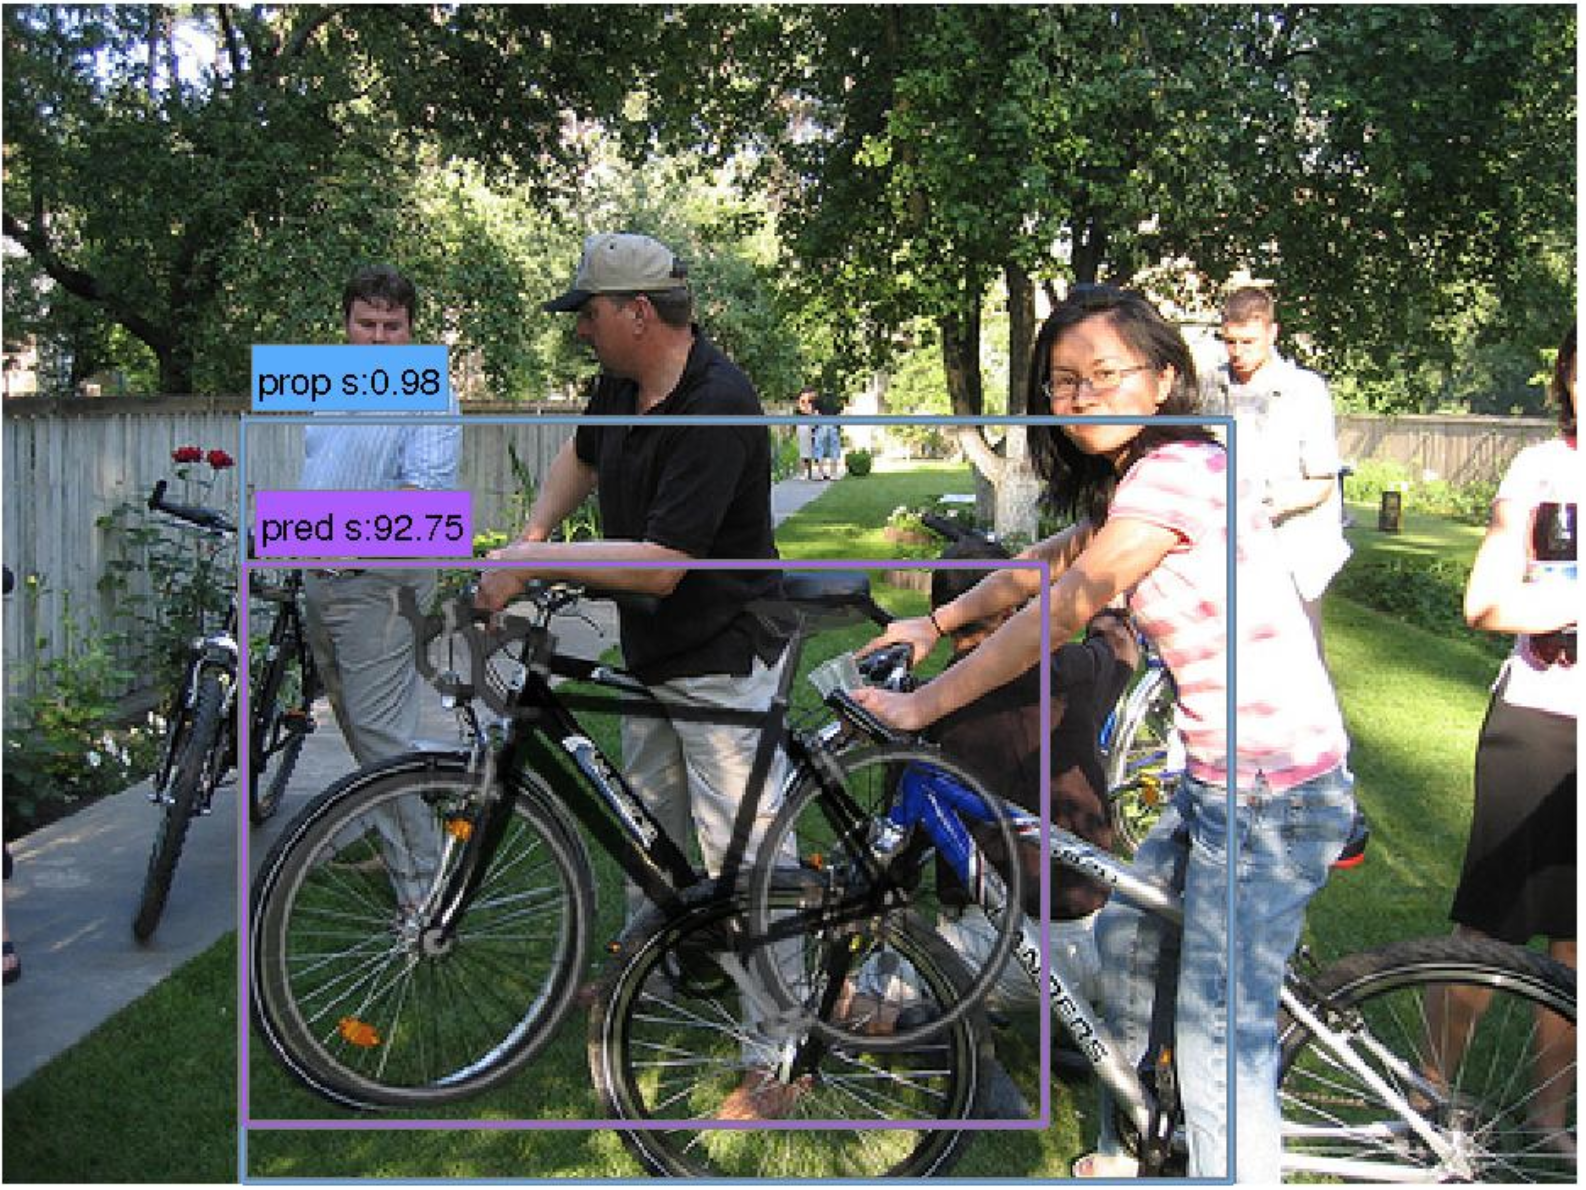
\includegraphics[width=0.18\textwidth]{bicycle_cnn/4c.png} \\
\end{tabular}
\caption{Example enriched bounding boxes. Given R-CNN
	detection bounding boxes, our method predicts the best 2D-3D
	registration given the bounding box input. Blue boxes are R-CNN output and
	purple boxes are the tightest bounding box enclosing predicted CAD model.}
\label{fig:pascal12cnn}
\end{figure}


\vspace{-0.1in}
\paragraph{Non-Zero Whitened Histograms of Orientations.} Many works that use
rendering do not take the background into account
when synthesizing and whitening to generate an LDA template~\cite{Aubry14}. Our NZ-WHO removes the
background region while whitening thus preventing irrelevant regions from
corrupting the foreground.

In addition, our NZ-WHO method uses Conjugate Gradient to greatly speeds up the LDA generation. We show that our uncalibrated NZ-WHO template performs on par
with a calibrated WHO template while being 100x faster to generate.

% Also, the residual from the Conjugate Gradient method (the norm of $y-Ax$ for
% $Ax = y$) is smaller than 
% that of Cholesky decomposition. 

\vspace{-0.1in}
\paragraph{Fine-Tuning using MCMC.} Due to the speed of our template synthesis
procedure, we are able to perform joint optimization of scale, translation,
continuous rotation, and focal length using the Metropolis-Hastings algorithm.

We model the probability of an object with the parameter $\theta$ in the test
image $\mathcal{I}$ as $P(\theta| \mathcal{I}) \sim e^{ \max_{s} w(\theta)
	\ast \mathcal{T}_s(\mathcal{I})}$. We approximate the MAP solution for $\theta$ by
drawing samples from the distribution $P(\theta | \mathcal{I})$, using the
Metropolis-Hastings algorithm.

\vspace{-0.1in}
\paragraph{Experiments} First, we verify that our NZ-WHO method delivers
performance that is at least on par with the original WHO
formulation~\cite{Hariharan12} in terms of accuracy, while at the same time
resulting in large computational savings.

Second, we demonstrate that our method can be used for multi-view
object class detection in isolation. It can be applied in a sliding
window fashion to deliver 2D bounding boxes and viewpoint
information. Our method is competitive with the state-of-the-art in this
case.

Finally, we show that our method can be used to complement the
detections provided by an existing object class detector, such
as DPM or R-CNN. In this case, we show a considerable performance improvement
compared to previous work in the task of joint object class detection and viewpoint
estimation. Example outputs of our model are in Fig.~\ref{fig:pascal12cnn}.

\vspace{-0.1in}
\paragraph{Acknowledgement.} We acknowledge the support of NSF CAREER grant
(N1054127), Ford-Stanford Innovation Alliance Award, DARPA, Korea Foundation
for Advanced Studies, Fulbright New Zealand and the Max Planck Center for Visual Computing \&
Communication.

\bibliography{egbib}

\end{document}
